\documentclass[12pt]{article}
\usepackage[utf8]{inputenc}
\usepackage{amsmath, amssymb, amsfonts}
\usepackage{amsthm}
\usepackage{graphicx}
\usepackage{hyperref}
\usepackage{geometry}
\usepackage{listings}
\usepackage{courier}
\usepackage{color}
\usepackage{enumitem}
\usepackage{caption}
\usepackage{float}
\usepackage{booktabs}
\usepackage{array}
\usepackage{minted}
\usepackage{seqsplit}

\geometry{letterpaper, margin=1in}

\lstset{
  basicstyle=\footnotesize\ttfamily,
  breaklines=true,
  columns=flexible,
  frame=single,
  numbers=left,
  numberstyle=\tiny,
  tabsize=2,
  keywordstyle=\color{blue},
  commentstyle=\color{gray},
  stringstyle=\color{red}
}



\title{Basketball Games Prediction Model Methodology}
\author{Jack Rubiralta, Jaden Patel, Kyan Hands, William Carten}
\date{\today}

\begin{document}
\maketitle
\pagebreak

%%%%%%%%%%%%%%%%%%%%%%%%%%%%%%%%%%%%%%%%%%%%%%%%%%%%%%%%%%%%%%%%%%%%%%%%%%%%%%%%%%%%%%%%%%%%%
% INTRODUCTION
%%%%%%%%%%%%%%%%%%%%%%%%%%%%%%%%%%%%%%%%%%%%%%%%%%%%%%%%%%%%%%%%%%%%%%%%%%%%%%%%%%%%%%%%%%%%%
\section{Introduction}
This document provides a technically rigorous explanation of a sports outcome prediction pipeline. We start from raw game data (stored in a CSV), transform it into meaningful features (including advanced statistics such as Strength-of-Schedule), and then construct a \textbf{stacking ensemble} of multiple machine learning models. This pipeline is designed to predict the probability that a given home team will win against a specific away team.

Key highlights and advanced topics covered:
\begin{itemize}[noitemsep]
    \item Detailed feature engineering: from raw box-score data to difference and ratio features
    \item In-depth theory and mathematical underpinnings of sub-models:
    \begin{enumerate}[label=\arabic*)]
        \item \textbf{XGBoost}: gradient boosting with advanced regularization
        \item \textbf{Random Forest}: bagging-based ensemble of decision trees
        \item \textbf{Logistic Regression}: convex optimization for meta-learning
    \end{enumerate}
    \item Advanced evaluation metrics (beyond accuracy, ROC AUC, log loss, Brier score)
    \item Hyperparameter optimization using \textbf{RandomizedSearchCV}
    \item Extended discussion of stacking ensemble theory and meta-learning synergy
\end{itemize}
\noindent
The repository where the code is stored: \url{https://github.com/JackRubiralta/sps-basketball-analytics}

%%%%%%%%%%%%%%%%%%%%%%%%%%%%%%%%%%%%%%%%%%%%%%%%%%%%%%%%%%%%%%%%%%%%%%%%%%%%%%%%%%%%%%%%%%%%%
% DATA INGESTION AND STRUCTURE
%%%%%%%%%%%%%%%%%%%%%%%%%%%%%%%%%%%%%%%%%%%%%%%%%%%%%%%%%%%%%%%%%%%%%%%%%%%%%%%%%%%%%%%%%%%%%
\section{Data Ingestion and Structure}
We assume a CSV file, \seqsplit{games\_data.csv}, where each row represents one team's performance in a particular game. Consequently, every actual game yields \emph{two} rows: one for the home team, one for the away team. Notable columns include:

\begin{itemize}[noitemsep]
    \item \seqsplit{game\_id, game\_date, team}: Identifiers for the game and the specific team.
    \item \seqsplit{FGA\_2, FGM\_2, FGA\_3, FGM\_3, FTA, FTM}: Basic box-score shooting stats (attempts and makes).
    \item \seqsplit{AST, BLK, STL, TOV}: Additional stats capturing assists, blocks, steals, and turnovers.
    \item \seqsplit{DREB, OREB, F\_personal}: Rebounds and personal fouls.
    \item \seqsplit{team\_score, opponent\_team\_score}: Final scoreboard result.
    \item \seqsplit{home\_away}: Categorical variable (\seqsplit{"home"} or \seqsplit{"away"}).
    \item \seqsplit{rest\_days, travel\_dist}: Additional context, e.g., how many days of rest a team had prior to this game and how far the team traveled.
\end{itemize}

\noindent
\textbf{Example CSV Rows:}
\begin{minted}[breaklines]{csv}
game_id,game_date,team,FGA_2,FGM_2,FGA_3,FGM_3,FTA,FTM,AST,BLK,STL,TOV,TOV_team,DREB,OREB,F_tech,F_personal,team_score,opponent_team_score,largest_lead,notD1_incomplete,OT_length_min_tot,rest_days,attendance,tz_dif_H_E,prev_game_dist,home_away,home_away_NS,travel_dist
game_2022_2011,12/30/2021,georgia_lady_bulldogs,50,22,11,5,6,3,14,7,7,18,0,25,11,0,18,62,68,1.0,False,,9.0,3241.0,0.0,0.0,home,1,0.0
game_2022_2011,12/30/2021,lsu_tigers,50,24,11,4,15,8,15,2,15,14,2,25,11,0,7,68,62,14.0,False,,3.0,3241.0,0.0,824.0,away,-1,824.0
\end{minted}
\subsection{Class \seqsplit{GamesData} for Data Management}
\seqsplit{GamesData} serves as a robust data handler:
\begin{enumerate}[label=\arabic*)]
    \item \textbf{Load CSV and Verify Existence}: Raises a \seqsplit{FileNotFoundError} if the path is invalid.
    \item \textbf{Compute Team Averages}: Aggregates basic stats across all games for each team.
    \item \textbf{Compute Win Percentage (\(\text{WP}\)) and Strength-of-Schedule (\(\text{SoS}\))}: 
        \begin{itemize}[noitemsep]
            \item \seqsplit{WP} = fraction of games won
            \item \seqsplit{SoS} = average WP of opponents
        \end{itemize}
    \item \textbf{Feature Column Definitions}: Maintains lists of columns (e.g., \seqsplit{\_cols\_to\_avg}) for constructing final features.
\end{enumerate}

Below is an excerpt showing how \seqsplit{GamesData} is initialized to accomplish this:

\begin{minted}[breaklines]{python}
def __init__(self, csv_path: str):
    if not os.path.exists(csv_path):
        raise FileNotFoundError(f"{csv_path} does not exist.")
    self.csv_path = csv_path
    self.df = pd.read_csv(csv_path)

    # Precompute the team averages (includes team_win_pct and team_sos)
    self.team_avgs = self._compute_team_averages(self.df)

    # We store the base set of columns for features:
    # (home_avg_*), (away_avg_*), plus rest/travel
    self.base_feature_cols = []
    ...
\end{minted}

\noindent
In this code:
\begin{itemize}
    \item We immediately \textbf{load the CSV} into a pandas DataFrame.
    \item We then \textbf{compute team-level averages} and advanced metrics (win percentage, SoS) by calling \seqsplit{\_compute\_team\_averages}.
    \item We also define lists of columns that will be used to build the final feature matrix.
\end{itemize}
%%%%%%%%%%%%%%%%%%%%%%%%%%%%%%%%%%%%%%%%%%%%%%%%%%%%%%%%%%%%%%%%%%%%%%%%%%%%%%%%%%%%%%%%%%%%%
% ADVANCED FEATURE ENGINEERING
%%%%%%%%%%%%%%%%%%%%%%%%%%%%%%%%%%%%%%%%%%%%%%%%%%%%%%%%%%%%%%%%%%%%%%%%%%%%%%%%%%%%%%%%%%%%%
\section{Advanced Feature Engineering}

\subsection{Team Averages, Win Percentage, SoS}
We group the data by \seqsplit{team} to compute:
\begin{align*}
\text{avg\_FGA\_2} &= \frac{1}{n}\sum \text{FGA\_2}, \\
\text{avg\_FGM\_2} &= \frac{1}{n}\sum \text{FGM\_2}, \quad \ldots
\end{align*}
where \(n\) is the total number of games for each team.

\subsubsection{Win Percentage (WP)}
For each row \(i\), define
\[
\text{win}_i = \mathbf{1}\{ \text{team\_score}_i > \text{opponent\_team\_score}_i \}.
\]
Then for team \(T\),
\[
\text{team\_win\_pct}_T = \frac{1}{n_T} \sum_{i=1}^{n_T} \text{win}_i.
\]

\subsubsection{Strength-of-Schedule (SoS)}
We define
\[
\text{SoS}_T = \frac{1}{n_T} \sum_{(T, O) \in \mathcal{G}} \text{team\_win\_pct}_O,
\]
where \(\mathcal{G}\) is the set of games in which team \(T\) faces an opponent \(O\). This provides a measure of difficulty of each team’s schedule.

\begin{minted}[breaklines]{python}
def _compute_team_averages(self, df: pd.DataFrame) -> pd.DataFrame:
    """
    1) Group by 'team' and compute mean of self._cols_to_avg (basic stats)
    2) Compute 'team_win_pct' for each team
    3) Compute 'team_sos' as the average (opponent_win_pct)
    4) Merge them all into a single DataFrame
    """
    # -- Compute average basic stats --
    df_avg = df.groupby("team")[self._cols_to_avg].mean().reset_index()

    # -- Compute "win" for each row, i.e. if team_score > opponent_team_score --
    df_temp = df.copy()
    df_temp["win"] = (df_temp["team_score"] > df_temp["opponent_team_score"]).astype(int)

    # -- Team-level win percentage --
    df_team_wp = (
        df_temp.groupby("team")["win"]
        .mean()
        .reset_index()
        .rename(columns={"win": "team_win_pct"})
    )

    ...
\end{minted}

\noindent
This snippet demonstrates:
\begin{enumerate}[label=\roman*)]
    \item How we compute the \emph{mean} of columns like \(\seqsplit{FGA\_2}\), \(\seqsplit{FGM\_2}\), etc.\@ per team.
    \item Assign an indicator \seqsplit{win} based on the scoreboard.
    \item Calculate each team's \seqsplit{team\_win\_pct} via the mean of \(\seqsplit{win}\).
\end{enumerate}
Further steps then identify each team's opponents and average their \(\seqsplit{win\_pct}\) to get \(\seqsplit{team\_sos}\).

\subsection{Merging Home and Away Rows}
To create a single row per actual game:
\begin{enumerate}[label=\arabic*)]
    \item Split the DataFrame into \(\mathbf{H}\) (home rows) and \(\mathbf{A}\) (away rows).
    \item Merge on \(\seqsplit{game\_id}\), creating columns with prefixes \(\text{home\_}\) and \(\text{away\_}\).
    \item The target label is 
    \[
    \text{home\_team\_won} = \mathbf{1}\{\text{home\_team\_score} > \text{away\_team\_score}\}.
    \]
\end{enumerate}

\begin{minted}[breaklines]{python}
def prepare_training_data(self) -> pd.DataFrame:
    """
    Merges home & away rows into one row per game, storing
    home_* stats, away_* stats, plus the label 'home_team_won'.
    """
    df_home = self.df[self.df["home_away"] == "home"].copy()
    df_away = self.df[self.df["home_away"] == "away"].copy()

    # Merge each side with the team averages
    df_home = df_home.merge(self.team_avgs, on="team", how="left")
    df_away = df_away.merge(self.team_avgs, on="team", how="left")

    # Rename columns to home_* or away_*
    ...
    merged = pd.merge(df_home, df_away, on="game_id", how="inner")

    # Label: did the home team win?
    merged["home_team_won"] = (merged["home_team_score"] > merged["away_team_score"]).astype(int)
    return merged
\end{minted}

\noindent
Here:
\begin{itemize}
    \item \seqsplit{df\_home} and \seqsplit{df\_away} subsets correspond to \seqsplit{home\_away == "home"} or \seqsplit{"away"}.
    \item We \emph{merge} them by \seqsplit{game\_id}, so each row in the final \seqsplit{merged} DataFrame holds data for one game.
    \item A binary label \seqsplit{home\_team\_won} is added for subsequent training.
\end{itemize}

\subsection{Difference and Ratio Features}
In advanced sports analytics, direct head-to-head metrics often matter more than raw values. We define:
\[
\text{diff\_X} = (\text{home\_X}) - (\text{away\_X}), 
\quad 
\text{ratio\_X} = \frac{\text{home\_X} + 10^{-6}}{\text{away\_X} + 10^{-6}}.
\]
Here, \(X\) can be any of \(\{ \text{avg\_AST}, \text{team\_win\_pct}, \text{team\_sos}, \ldots \}\). The small constant avoids division by zero. Below is an example illustrating how these features are appended:

\begin{minted}[breaklines]{python}
def get_feature_and_label_arrays(self, merged_df: pd.DataFrame, 
                                 label_col: str = "home_team_won"):
    # 1) Base features
    X_base = merged_df[self.base_feature_cols].values
    y = merged_df[label_col].values

    # 2) Create difference & ratio features
    diff_ratio_features = []
    n_stats = len(self._stats_for_diff)

    for i_row in range(X_base.shape[0]):
        row_vals = X_base[i_row]
        row_diff_ratio = []
        for i_stat in range(n_stats):
            home_val = row_vals[i_stat]
            away_val = row_vals[n_stats + i_stat]

            diff = home_val - away_val
            ratio = (home_val + 1e-6) / (away_val + 1e-6)

            row_diff_ratio.append(diff)
            row_diff_ratio.append(ratio)
        diff_ratio_features.append(row_diff_ratio)

    diff_ratio_features = np.array(diff_ratio_features, dtype=np.float32)
    X = np.concatenate([X_base, diff_ratio_features], axis=1)

    return X, y
\end{minted}

\noindent
\textbf{Key Points:}
\begin{itemize}
    \item We first extract \seqsplit{X\_base} from columns like \seqsplit{home\_avg\_FGA\_2}, \seqsplit{away\_avg\_FGA\_2}, \seqsplit{home\_team\_win\_pct}, etc.
    \item We compute \(\seqsplit{diff\_X}\) and \(\seqsplit{ratio\_X}\) for each relevant statistical category.
    \item Finally, we concatenate these difference/ratio columns to the end of \seqsplit{X\_base}.
\end{itemize}

%%%%%%%%%%%%%%%%%%%%%%%%%%%%%%%%%%%%%%%%%%%%%%%%%%%%%%%%%%%%%%%%%%%%%%%%%%%%%%%%%%%%%%%%%%%%%
% MODELING METHODOLOGY: STACKING ENSEMBLE
%%%%%%%%%%%%%%%%%%%%%%%%%%%%%%%%%%%%%%%%%%%%%%%%%%%%%%%%%%%%%%%%%%%%%%%%%%%%%%%%%%%%%%%%%%%%%
\section{Modeling Methodology: Stacking Ensemble}
Stacking (also known as stacked generalization) is an ensemble technique that combines diverse base learners (Level-0 models) via a meta-learner (Level-1 model). If each base learner has unique biases and variance characteristics, a well-tuned meta-learner can exploit these differences to produce superior generalization.

\subsection{Sub-Model A: XGBoost (Advanced Gradient Boosting)}

\subsubsection{Gradient Boosting Theory}
Let \(\{(x_i, y_i)\}_{i=1}^N\) be our training set with \(x_i \in \mathbb{R}^d\) and \(y_i \in \{0,1\}\). In gradient boosting, we fit an additive model of the form:
\[
F_0(x) = \arg\min_\gamma \sum_{i=1}^N \ell(y_i, \gamma),
\]
and iteratively update
\[
F_m(x) = F_{m-1}(x) + \nu \cdot h_m(x),
\]
where \(h_m\) is a weak learner (usually a small decision tree), and \(\nu\) is the learning rate. The function \(h_m\) is trained to fit the negative gradient of the loss function w.r.t. the current model.

\subsubsection{XGBoost-Specific Enhancements}
XGBoost (eXtreme Gradient Boosting) extends gradient boosting with:
\begin{itemize}[noitemsep]
    \item \textbf{Second-order approximations of the loss} for tree splitting: This uses both first- and second-order derivatives to select the best split (rather than just first-order).
    \item \textbf{Regularization Terms}: XGBoost adds \(L_1\) (Lasso) and \(L_2\) (Ridge) regularization on the leaf weights, effectively controlling model complexity. This is parameterized by \(\seqsplit{reg\_alpha}\) and \(\seqsplit{reg\_lambda}\).
    \item \textbf{Column Subsampling} (\(\seqsplit{colsample\_bytree}\)): Helps reduce correlation among trees.
    \item \textbf{Efficient Implementation}: Designed for high performance, leveraging out-of-core computation if necessary.
\end{itemize}

\subsubsection{Key Parameters}
\begin{itemize}[noitemsep]
    \item \(\seqsplit{n\_estimators}\): Number of boosting rounds (trees).
    \item \(\seqsplit{max\_depth}\): Maximum depth of each tree (controls model expressiveness).
    \item \(\seqsplit{learning\_rate}\) (\(\nu\)): Shrinks the contribution of each new tree.
    \item \(\gamma\) (or \(\seqsplit{min\_split\_loss}\)): Minimum loss reduction required for a partition to occur (discourages overfitting).
\end{itemize}

\begin{minted}[breaklines]{python}
# Excerpt showing XGBoost creation in Model.generate_model
xgb_clf = XGBClassifier(
    eval_metric='logloss',
    random_state=42,
)
\end{minted}

\noindent In the above snippet, we instantiate our XGBoost classifier with a specific \(\seqsplit{eval\_metric='logloss'}\) and a fixed \(\seqsplit{random\_state}\). This ensures reproducibility and that the final objective is aligned with typical binary classification (log loss).

\subsection{Sub-Model B: Random Forest (Bagging Ensemble of Trees)}

\subsubsection{Bagging and Decision Trees}
\textbf{Bagging} (Bootstrap Aggregating) is an approach where each tree is trained on a bootstrap sample (random sample with replacement) from the training set. Decision trees themselves partition feature space into axis-aligned regions. By aggregating (averaging) multiple such trees:
\begin{itemize}[noitemsep]
    \item We reduce variance, as each tree has a different view of the data.
    \item We preserve low bias, since large trees can approximate complex functions.
\end{itemize}

\subsubsection{Random Forest Enhancements}
Breiman’s Random Forest introduces further randomness by randomly selecting a subset of features at each split (controlled by \(\seqsplit{max\_features}\)). This mechanism reduces correlation among trees, often improving generalization.

\subsubsection{Key Parameters}
\begin{itemize}[noitemsep]
    \item \(\seqsplit{n\_estimators}\): Number of trees.
    \item \(\seqsplit{max\_depth}\): A limit on tree depth to prevent excessive overfitting.
    \item \(\seqsplit{max\_features}\): Determines how many features are considered at each split (e.g., \(\sqrt{d}\) or \(\log_2 d\)).
\end{itemize}

\begin{minted}[breaklines]{python}
# Excerpt showing Random Forest creation in Model.generate_model
rf_clf = RandomForestClassifier(random_state=42)
\end{minted}

\noindent Here, we see how the \(\seqsplit{RandomForestClassifier}\) is created with a fixed \(\seqsplit{random\_state}\). Additional parameters (like \(\seqsplit{n\_estimators}\) or \(\seqsplit{max\_depth}\)) can be passed or tuned via hyperparameter searches.

\subsection{Meta-Learner: Logistic Regression}

\subsubsection{Logistic Regression and Convex Optimization}
For binary classification, logistic regression fits the parameters \(\beta\) by minimizing the negative log-likelihood:
\[
\min_{\beta} \left[ -\sum_{i=1}^N \left\{ y_i \ln \sigma(z_i) + (1 - y_i)\ln [1 - \sigma(z_i)] \right\} \right],
\]
where \(z_i = \beta_0 + \sum_{j=1}^k \beta_j x_{ij}\) and \(\sigma(\cdot)\) is the sigmoid function. In the stacking context, \(x_{ij}\) are the predicted probabilities from the base models.

\subsubsection{Why Logistic Regression is an Excellent Meta-Learner}
\begin{enumerate}[label=\arabic*)]
    \item \textbf{Calibrated Probabilities}: Logistic regression naturally produces well-calibrated probability outputs, provided the training set is representative.
    \item \textbf{Low Variance, High Interpretability}: It has relatively low variance and a well-understood convex loss surface. The learned coefficients can be inspected to see how heavily each sub-model influences the final prediction.
    \item \textbf{Simplicity in High-Level Model Architecture}: Minimizes overfitting risk at the meta-level, ensuring each base model’s predictions are used in a way that improves generalization.
\end{enumerate}

\begin{minted}[breaklines]{python}
# Excerpt showing Logistic Regression creation in Model.generate_model
meta_learner = LogisticRegression(max_iter=2000)
\end{minted}

\noindent We specify \(\seqsplit{max\_iter=2000}\) to ensure logistic regression has enough iterations to converge, especially with potentially complex stacking outputs.

\subsection{Stacking Mechanism and Synergy}
Once the base models (XGBoost, Random Forest) are trained, the meta-learner (Logistic Regression) is fit on:
\[
\big\{ (p_{\text{xgb},i}, p_{\text{rf},i}),\, y_i \big\}_{i=1}^N,
\]
where \(p_{\text{xgb},i}, p_{\text{rf},i}\) are the predicted probabilities of a positive class from XGBoost and Random Forest, respectively, for sample \(i\).

If XGBoost systematically underestimates certain patterns but Random Forest overestimates them, logistic regression may find an appropriate weighting scheme for combining these predictions. By learning a linear combination (plus intercept) of these base outputs, the model can correct biases and exploit synergy between the learners.

\subsection{Example: Constructing the Stacking Classifier in Code}
Below, we show a snippet from the \seqsplit{Model.generate\_model} method that builds the \seqsplit{StackingClassifier} with XGBoost, Random Forest, and Logistic Regression. Note that some lines are omitted for brevity:

\begin{minted}[breaklines]{python}
def generate_model(self, do_hyperparam_search=True):
    # 1) Prepare data
    merged_df = self.games_data.prepare_training_data()
    X, y = self.games_data.get_feature_and_label_arrays(merged_df)

    X_train, X_test, y_train, y_test = train_test_split(
        X, y, test_size=0.2, stratify=y, random_state=42
    )

    # 2) Define base estimators
    xgb_clf = XGBClassifier(eval_metric='logloss', random_state=42)
    rf_clf  = RandomForestClassifier(random_state=42)
    meta_learner = LogisticRegression(max_iter=2000)

    # 3) Potential hyperparam search omitted here...
    
    # 4) Build stacking classifier
    estimators = [
        ('xgb', xgb_clf),
        ('rf', rf_clf)
    ]
    stack_clf = StackingClassifier(
        estimators=estimators,
        final_estimator=meta_learner,
        cv=5,
        n_jobs=-1,
        passthrough=False
    )

    # 5) Train stacking
    stack_clf.fit(X_train, y_train)
    self.model = stack_clf
\end{minted}

\noindent
\textbf{Key Observations}:
\begin{itemize}
    \item Two base learners: \(\seqsplit{xgb\_clf}\) (XGBClassifier) and \(\seqsplit{rf\_clf}\) (RandomForestClassifier).
    \item \seqsplit{final\_estimator} is \(\seqsplit{meta\_learner}\), i.e., logistic regression.
    \item By setting \(\seqsplit{cv}=5\), we use 5-fold cross-validation to generate out-of-fold predictions for stacking.
    \item We assign \(\seqsplit{self.model} = \seqsplit{stack\_clf}\) so the final stacked model is accessible throughout the class.
\end{itemize}

%%%%%%%%%%%%%%%%%%%%%%%%%%%%%%%%%%%%%%%%%%%%%%%%%%%%%%%%%%%%%%%%%%%%%%%%%%%%%%%%%%%%%%%%%%%%%
% HYPERPARAMETER OPTIMIZATION
%%%%%%%%%%%%%%%%%%%%%%%%%%%%%%%%%%%%%%%%%%%%%%%%%%%%%%%%%%%%%%%%%%%%%%%%%%%%%%%%%%%%%%%%%%%%%
\section{Hyperparameter Optimization}

\subsection{Randomized Search \emph{vs.} Grid Search}
We use \textbf{RandomizedSearchCV} due to the relatively large hyperparameter space in XGBoost and Random Forest. Randomized search:
\begin{itemize}[noitemsep]
    \item Provides more exploration of the parameter space in fewer iterations compared to an exhaustive grid.
    \item Prevents us from having to try every possible combination, many of which can be infeasible or unnecessary.
\end{itemize}

\subsection{Cross-Validation Scheme}
The pipeline uses \(k\)-fold (e.g., 3- or 5-fold) cross-validation to evaluate each parameter setting. Each fold’s data acts as a local hold-out set, ensuring robust estimation of out-of-sample performance.

\subsection{Performance Metric: ROC AUC \emph{vs.} Others}
We often optimize ROC AUC (\(\seqsplit{scoring='roc\_auc'}\)). Alternatives include:
\begin{itemize}[noitemsep]
    \item \textbf{Average Precision} (for imbalanced data).
    \item \textbf{Log Loss} (if probability calibration is paramount).
\end{itemize}

\subsection{Code Excerpt: Hyperparameter Search}
Below is a more extensive excerpt showing how one might incorporate \seqsplit{RandomizedSearchCV} for XGBoost and Random Forest within \seqsplit{generate\_model}. This demonstrates how the \emph{best} hyperparameters are selected and the resulting estimators are used in the stacking:

\begin{minted}[breaklines]{python}
if do_hyperparam_search:
    # Hyperparameters for XGB
    xgb_params = {
        "n_estimators":    [100, 200, 300, 500],
        "max_depth":       [3, 4, 6, 8],
        "learning_rate":   [0.01, 0.05, 0.1],
        "subsample":       [0.6, 0.8, 1.0],
        "colsample_bytree":[0.6, 0.8, 1.0],
        "gamma":           [0, 0.1, 0.2],
        "reg_lambda":      [1, 2, 5],
        "reg_alpha":       [0, 0.1, 1]
    }
    xgb_search = RandomizedSearchCV(
        estimator=xgb_clf,
        param_distributions=xgb_params,
        n_iter=10,  # can increase for more thorough search
        scoring='roc_auc',
        cv=3,
        random_state=42,
        n_jobs=-1,
        verbose=1
    )
    xgb_search.fit(X_train, y_train)
    xgb_clf = xgb_search.best_estimator_
    print("Best XGB params:", xgb_search.best_params_)

    # Hyperparameters for Random Forest
    rf_params = {
        "n_estimators": [100, 200, 500],
        "max_depth":    [None, 5, 10, 20],
        "max_features": ["sqrt", "log2", None]
    }
    rf_search = RandomizedSearchCV(
        estimator=rf_clf,
        param_distributions=rf_params,
        n_iter=5,
        scoring='roc_auc',
        cv=3,
        random_state=42,
        n_jobs=-1,
        verbose=1
    )
    rf_search.fit(X_train, y_train)
    rf_clf = rf_search.best_estimator_
    print("Best RF params:", rf_search.best_params_)
\end{minted}

\noindent
\textbf{Summary of Key Steps}:
\begin{itemize}
    \item \textbf{Parameter dictionaries} define potential values for \(\seqsplit{XGBClassifier}\) and \(\seqsplit{RandomForestClassifier}\).
    \item \(\seqsplit{RandomizedSearchCV}\) iterates over a subset of these values, using cross-validation (here, \(\seqsplit{cv=3}\)) to assess performance.
    \item The best-found estimators are stored back into \(\seqsplit{xgb\_clf}\) and \(\seqsplit{rf\_clf}\) for use in stacking.
\end{itemize}

%%%%%%%%%%%%%%%%%%%%%%%%%%%%%%%%%%%%%%%%%%%%%%%%%%%%%%%%%%%%%%%%%%%%%%%%%%%%%%%%%%%%%%%%%%%%%
% EVALUATION AND DIAGNOSTICS
%%%%%%%%%%%%%%%%%%%%%%%%%%%%%%%%%%%%%%%%%%%%%%%%%%%%%%%%%%%%%%%%%%%%%%%%%%%%%%%%%%%%%%%%%%%%%
\section{Evaluation and Diagnostics}

\subsection{Standard Metrics}
\begin{itemize}[noitemsep]
    \item \textbf{Accuracy}: 
    \[
    \text{Accuracy} = \frac{\text{correct predictions}}{\text{total}}
    \]
    \item \textbf{ROC AUC}: Probability the model ranks a random positive higher than a random negative. 
    \item \textbf{Log Loss}: Measures the “confidence” of correct vs. incorrect predictions. Lower is better.
    \item \textbf{Brier Score}: 
    \[
    \text{Brier} = \frac{1}{N} \sum_{i=1}^N (\hat{p}_i - y_i)^2
    \]
    Also used to judge calibration quality.
\end{itemize}

\subsection{Calibration Considerations}
For probabilistic outputs, we examine calibration plots. A well-calibrated model implies that among all test samples where \(\hat{p} = p\), approximately \(p \times 100\%\) of them actually have \(y=1\). This is critical if the predictions are used in a decision-making context (e.g., betting markets or resource allocation).

%%%%%%%%%%%%%%%%%%%%%%%%%%%%%%%%%%%%%%%%%%%%%%%%%%%%%%%%%%%%%%%%%%%%%%%%%%%%%%%%%%%%%%%%%%%%%
% DEPLOYMENT AND PREDICTION USE CASES
%%%%%%%%%%%%%%%%%%%%%%%%%%%%%%%%%%%%%%%%%%%%%%%%%%%%%%%%%%%%%%%%%%%%%%%%%%%%%%%%%%%%%%%%%%%%%
\section{Deployment and Prediction Use Cases}

\subsection{Single-Game Prediction}
To predict a single future matchup:
\begin{enumerate}[label=\roman*)]
    \item Retrieve the aggregated stats (\(\text{avg\_FGA\_2}\), \(\text{team\_win\_pct}\), etc.) for both home and away teams.
    \item Incorporate rest days, travel distance, or any other contextual features.
    \item Construct difference/ratio features.
    \item Pass the resulting feature vector through the stacking ensemble’s \seqsplit{predict\_proba}.
    \item Output the final probability that the home team wins.
\end{enumerate}

\subsubsection{Illustrative Code for Single-Game Prediction}
Below is how \seqsplit{predict\_single\_game} might be implemented within our \seqsplit{Model} class, showcasing the creation of a single-row feature vector. We see how the synergy of \(\seqsplit{build\_prediction\_features}\) ensures consistent feature engineering:

\begin{minted}[breaklines]{python}
def predict_single_game(self, team_home: str, team_away: str,
                        home_rest_days: float, home_travel_dist: float,
                        away_rest_days: float, away_travel_dist: float) -> float:
    """
    Returns the predicted probability that the home team wins.
    """
    if self.model is None:
        raise ValueError("No model loaded or trained. Please train or load a model first.")

    X_single = self.games_data.build_prediction_features(
        team_home, team_away,
        home_rest_days, home_travel_dist,
        away_rest_days, away_travel_dist
    )
    prob = self.model.predict_proba(X_single)[:, 1][0]
    return prob
\end{minted}

\noindent
\textbf{Key Observations:}
\begin{itemize}
    \item We generate a single-row feature vector with \(\seqsplit{games\_data.build\_prediction\_features}\), preserving the same structure used during training.
    \item \(\seqsplit{predict\_proba}\) yields class probabilities, of which the second column is the probability of \(\seqsplit{home\_team\_won} = 1\).
\end{itemize}

\subsection{Batch Predictions}
For large-scale forecasting (e.g., entire tournament brackets):
\begin{itemize}[noitemsep]
    \item Construct a matrix \(\mathbf{X}_{\text{new}}\) with each row corresponding to a new matchup.
    \item Use \(\seqsplit{model.predict\_batch}(\mathbf{X}_{\text{new}})\) to retrieve an array of probabilities.
    \item Optionally apply domain-specific thresholds or post-processing.
\end{itemize}

\subsubsection{Batch Prediction Code Example}
If you have already built your feature matrix \(\mathbf{X}_{\text{new}}\), you can simply call:

\begin{minted}[breaklines]{python}
def predict_batch(self, X: np.ndarray) -> np.ndarray:
    """
    For batch predictions where X is already constructed,
    returns predicted probabilities for the home team.
    """
    if self.model is None:
        raise ValueError("No model found. Please train or load a model.")
    return self.model.predict_proba(X)[:, 1]
\end{minted}

\noindent
This method bypasses the repeated feature engineering steps because it expects \(\mathbf{X}\) to be in the exact format used during training. This is especially handy for large-scale or repeated forecasts.
%%%%%%%%%%%%%%%%%%%%%%%%%%%%%%%%%%%%%%%%%%%%%%%%%%%%%%%%%%%%%%%%%%%%%%%%%%%%%%%%%%%%%%%%%%%%%
% EVALUATION AND TESTING
%%%%%%%%%%%%%%%%%%%%%%%%%%%%%%%%%%%%%%%%%%%%%%%%%%%%%%%%%%%%%%%%%%%%%%%%%%%%%%%%%%%%%%%%%%%%%
%%%%%%%%%%%%%%%%%%%%%%%%%%%%%%%%%%%%%%%%%%%%%%%%%%%%%%%%%%%%%%%%%%%%%%%%%%%%%%%%%%%%%%%%%%%%%
% EVALUATION AND TESTING
%%%%%%%%%%%%%%%%%%%%%%%%%%%%%%%%%%%%%%%%%%%%%%%%%%%%%%%%%%%%%%%%%%%%%%%%%%%%%%%%%%%%%%%%%%%%%
\section{Evaluation and Testing}
\label{sec:evaluation_testing}
\subsection{Testing Methodology and Code Excerpts}
To ensure consistency and rigorous evaluation, our testing procedure is implemented in a script called \seqsplit{test\_model.py}. Below we describe the core steps:

\subsubsection{Data Preparation and Model Loading}
We initialize the feature-engineering object \seqsplit{GamesData} and then load (or train) a stacking model via the \seqsplit{Model} class:
\begin{minted}[breaklines]{python}
training_csv_path = "games_data.csv"
games_data = GamesData(training_csv_path)

model_file_path = "model_stuff.json"
my_model = Model(model_file_path=model_file_path, games_data=games_data)
if my_model.model is None:
    raise ValueError(f"No model loaded from {model_file_path}.")
\end{lstlisting}

\subsubsection{Evaluation on a Held-Out Test Split}
The main testing flow:
\begin{enumerate}[label=\arabic*)]
    \item \textbf{Prepare merged data}, including \seqsplit{point\_diff} for analysis.
    \item \textbf{Build feature matrix} \(X\) and label vector \(y\).
    \item \textbf{Split into training and testing} sets with 80--20 partition (stratified by \(y\)).
    \item \textbf{Predict} on the test set and \textbf{compute metrics}.
\end{enumerate}

\begin{minted}[breaklines]{python}
merged_df = games_data.prepare_training_data()
merged_df["point_diff"] = merged_df["home_team_score"] - merged_df["away_team_score"]

X, y = games_data.get_feature_and_label_arrays(merged_df)
diff_array = merged_df["point_diff"].values

X_train, X_test, y_train, y_test, diff_train, diff_test = train_test_split(
    X, y, diff_array,
    test_size=0.2,
    stratify=y,
    random_state=42
)

y_probs = my_model.predict_batch(X_test)
y_pred  = (y_probs >= 0.5).astype(int)
\end{minted}

\noindent
Metrics such as Accuracy, Brier Score, Log Loss, and ROC AUC are calculated, and a confusion matrix or classification report is generated.

%%%%%%%%%%%%%%%%%%%%%%%%%%%%%%%%%%%%%%%%%%%%%%%%%%%%%%%%%%%%%%%%%%%%%%%%%%%%%%%%%%%%%%%%%%%%%
% RESULTS
%%%%%%%%%%%%%%%%%%%%%%%%%%%%%%%%%%%%%%%%%%%%%%%%%%%%%%%%%%%%%%%%%%%%%%%%%%%%%%%%%%%%%%%%%%%%%
\section{Results}
\subsection{Overall Results and Accuracy}

\noindent
\textbf{Numerical Results:}
\[
\begin{bmatrix}
\text{TN} = 262 & \text{FP} = 134 \\
\text{FN} = 71  & \text{TP} = 516
\end{bmatrix}.
\]
The model achieves an \(\textbf{accuracy} \approx 79\%\). Formally, accuracy is:
\[
\text{Accuracy} \;=\; \frac{\text{TP} + \text{TN}}{\text{TP} + \text{TN} + \text{FP} + \text{FN}},
\]
where \(\text{TP}, \text{TN}, \text{FP}, \text{FN}\) are true positives, true negatives, false positives, and false negatives, respectively.

\paragraph{Overall Performance.}
An accuracy of \(\approx 79\%\) indicates that the model robustly discriminates between home and away wins. The confusion matrix reveals that the model correctly identifies \(\text{TP} = 516\) home-team wins and \(\text{TN} = 262\) away-team wins, with moderate false positives (\(\text{FP} = 134\)) and false negatives (\(\text{FN} = 71\)). Depending on the use case (e.g., betting vs.\ general analytics), one could adjust the probability threshold to prioritize reducing false positives or false negatives.

\subsection{ROC Curve and AUC}

\begin{figure}[H]
\centering
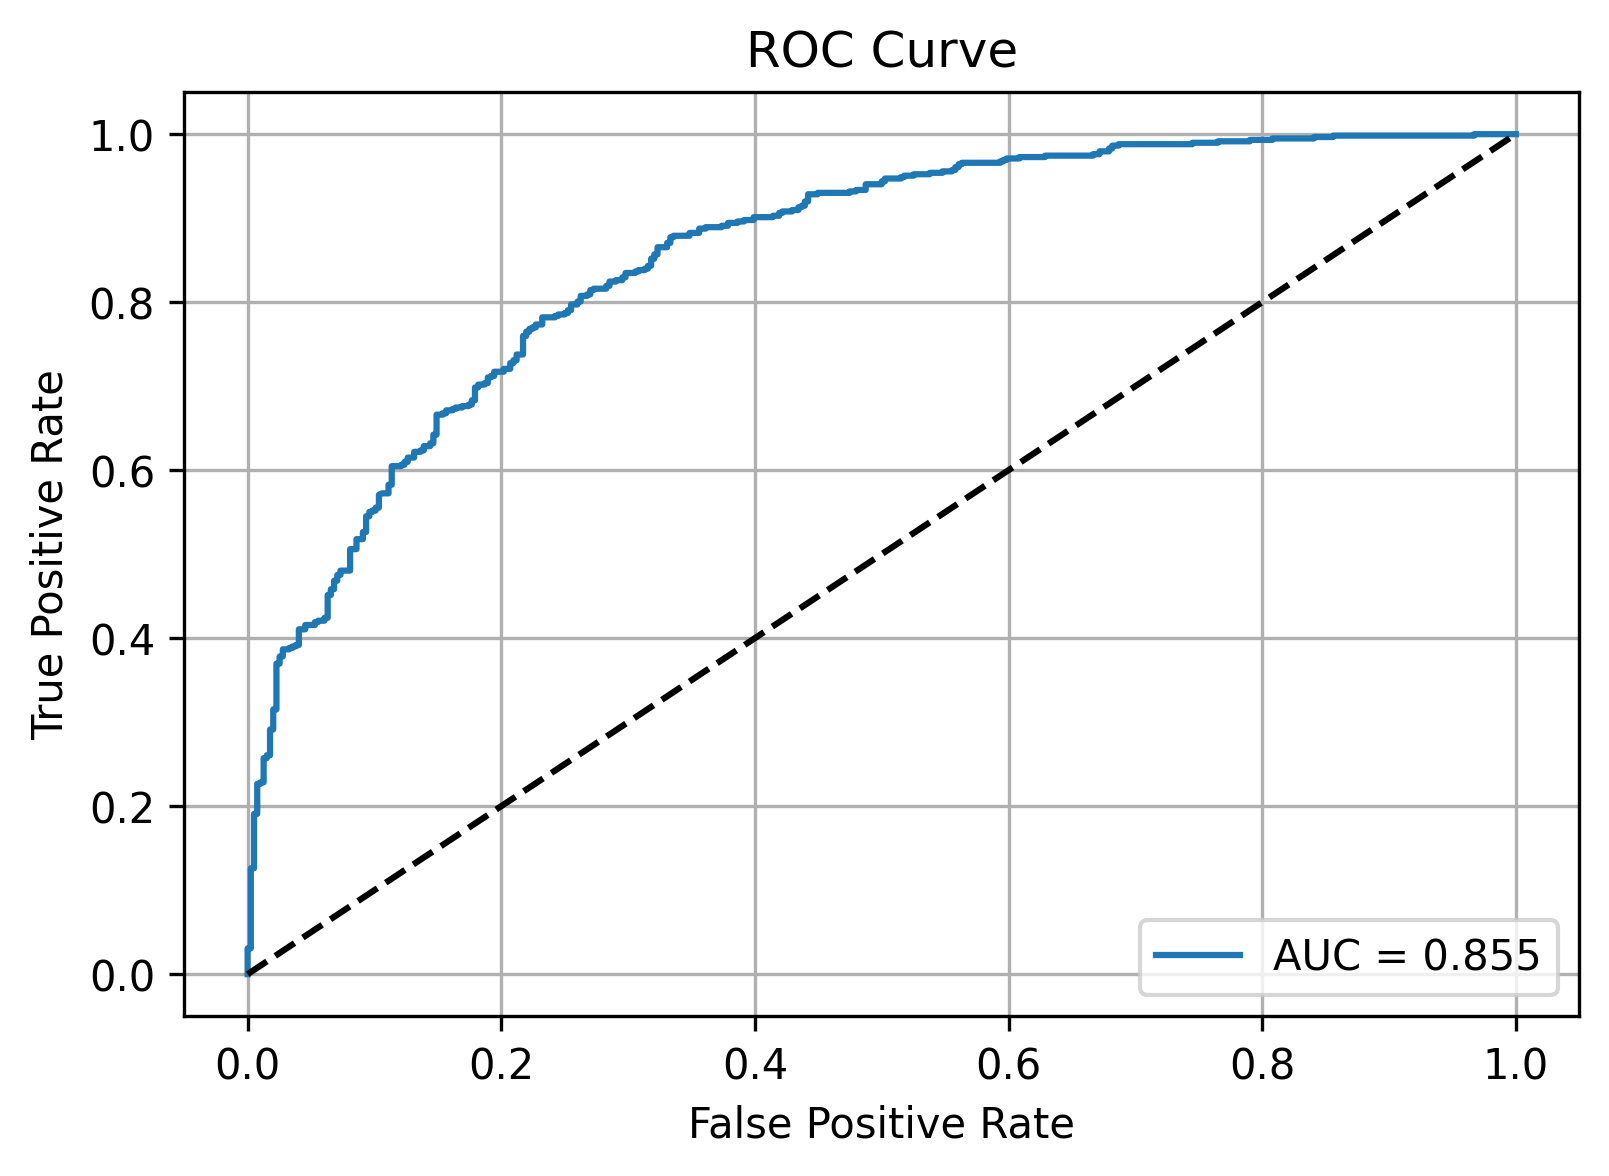
\includegraphics[width=0.5\textwidth]{graph_roc_curve.png}
\caption{ROC Curve (AUC = 0.855). The diagonal line represents a random classifier.}
\label{fig:roc_curve}
\end{figure}

\noindent
\textbf{Numerical Result:} \(\text{ROC AUC} = 0.855.\)

\paragraph{Analysis.}
The ROC curve plots the \textit{True Positive Rate} (TPR) against the \textit{False Positive Rate} (FPR) at various classification thresholds. Formally,
\[
\text{TPR} = \frac{\text{TP}}{\text{TP} + \text{FN}}, 
\quad
\text{FPR} = \frac{\text{FP}}{\text{FP} + \text{TN}}.
\]
An \(\text{AUC} = 0.855\) indicates that the model can correctly rank a randomly chosen positive instance (home-team win) above a randomly chosen negative instance (away-team win) roughly 85.5\% of the time. This is a strong result, showing that the classifier is well above the random-guessing baseline (\(\text{AUC} = 0.5\)).

\subsection{Calibration Plot and Brier Score}

\begin{figure}[H]
\centering
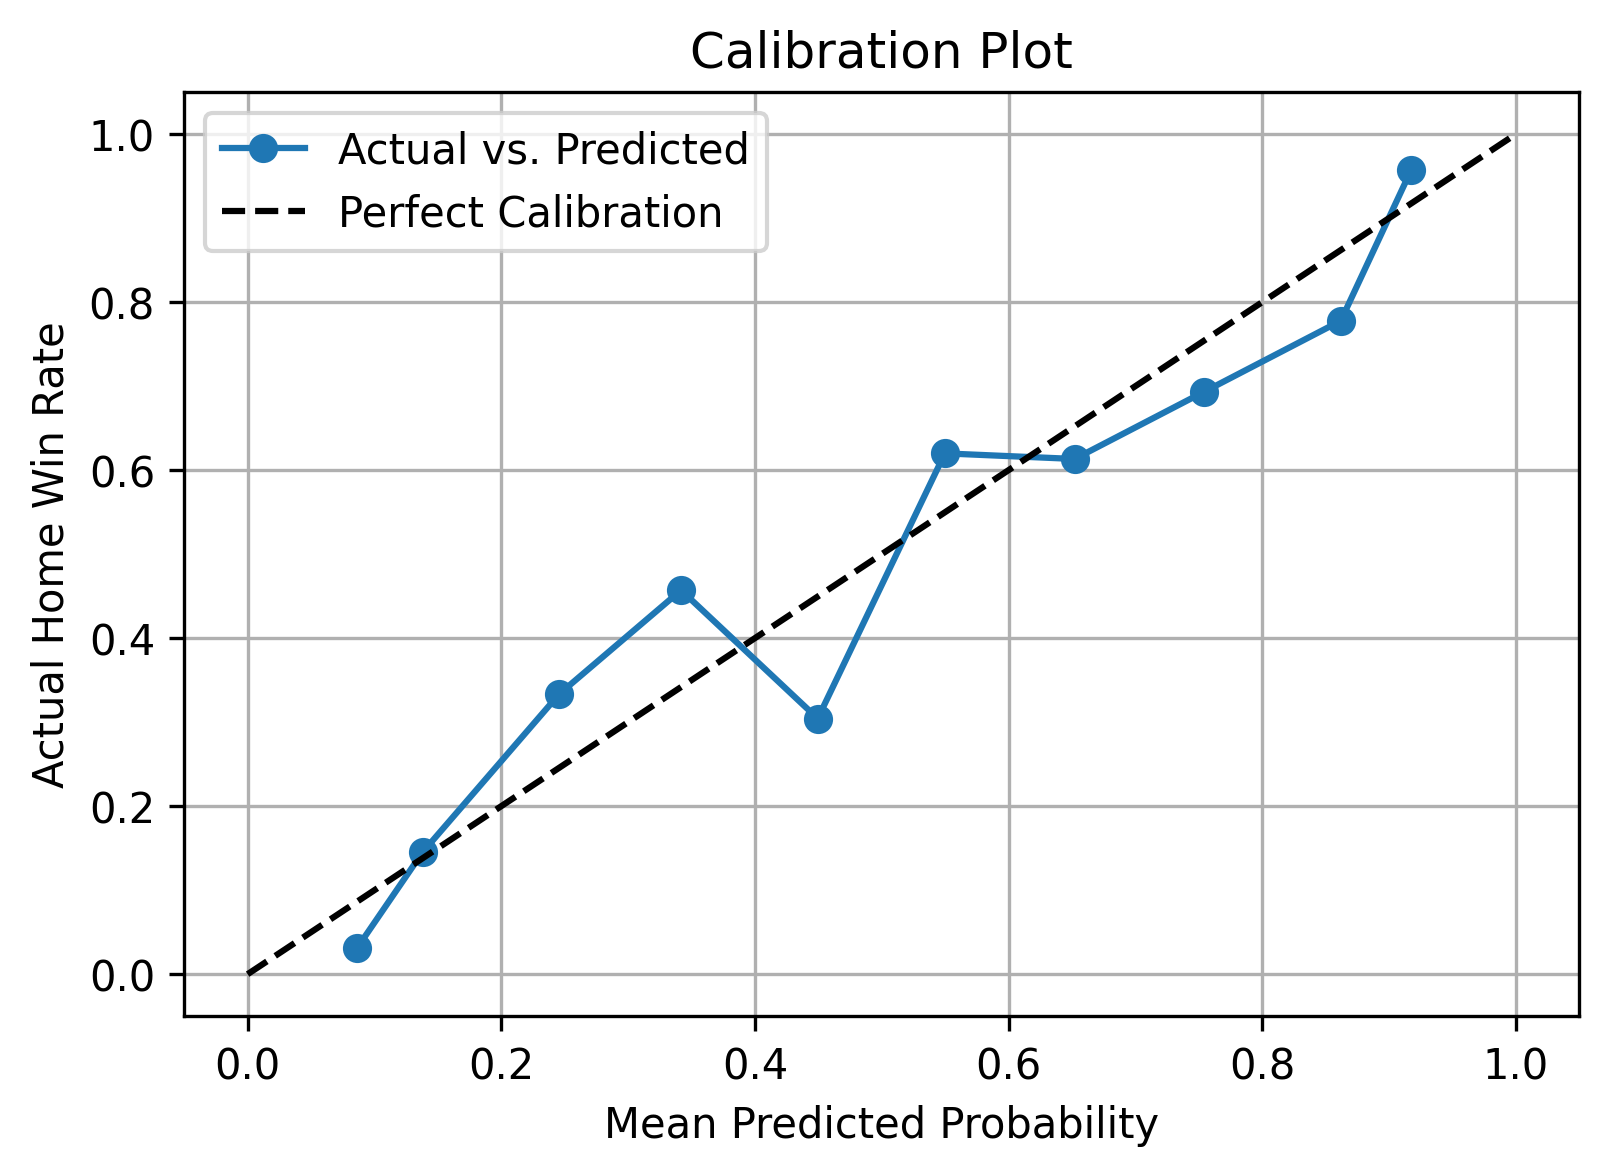
\includegraphics[width=0.5\textwidth]{graph_calibration.png}
\caption{Calibration Plot: Actual Home Win Rate vs.\ Mean Predicted Probability.}
\label{fig:calibration}
\end{figure}

\noindent
\textbf{Numerical Result:} \(\text{Brier Score} = 0.1523.\)

\paragraph{Probability Calibration.}
The calibration plot compares the model’s predicted probabilities to the observed frequency of home-team wins. Perfect calibration would lie on the diagonal (dashed line). Our model’s curve is reasonably close to that diagonal, indicating that when the model predicts a probability \(p\), the long-run fraction of actual home-team wins is close to \(p\). This is further quantified by the Brier Score:
\[
\text{Brier Score} 
\;=\;
\frac{1}{N}\sum_{i=1}^N (\hat{p}_i - y_i)^2,
\]
where \(\hat{p}_i\) is the predicted probability of a home-team win for instance \(i\), and \(y_i \in \{0,1\}\) is the true outcome. A value of \(0.1523\) is relatively low, indicating strong calibration performance.

\subsection{Distribution of Predictions}

\begin{figure}[H]
\centering
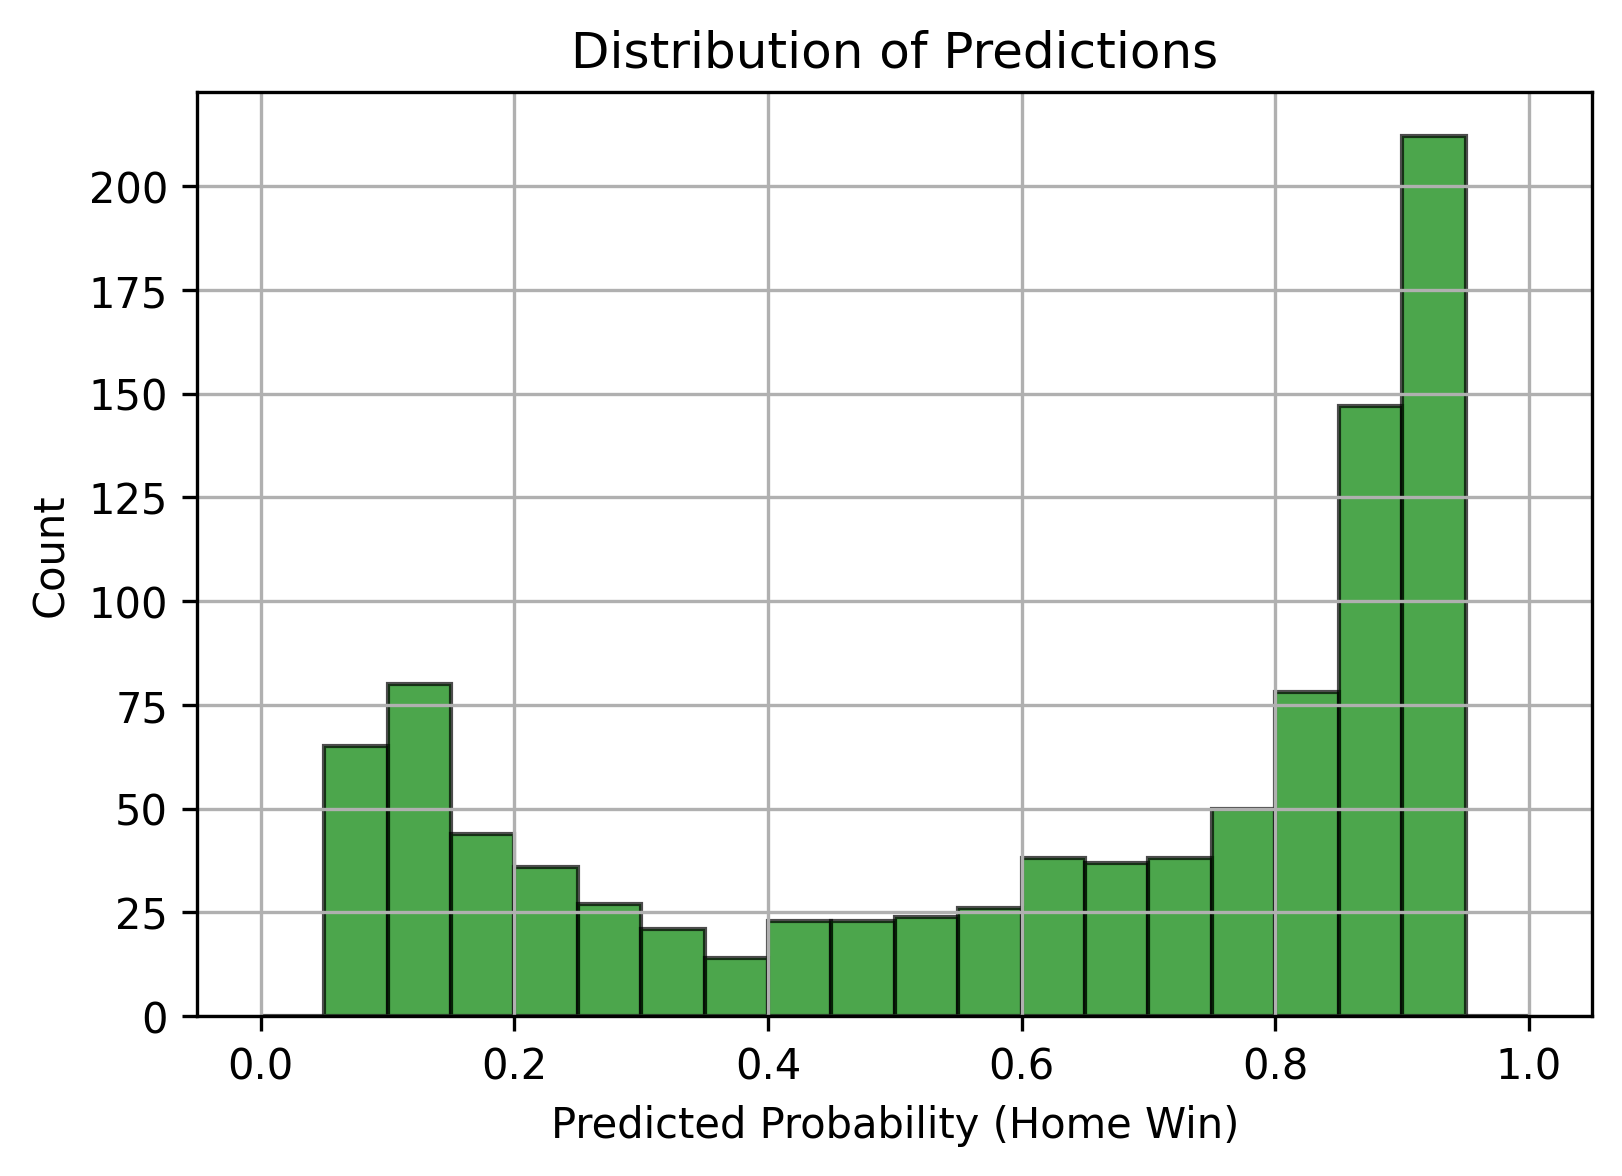
\includegraphics[width=0.5\textwidth]{graph_histogram.png}
\caption{Distribution of Predicted Probabilities (Home Win).}
\label{fig:distribution_predictions}
\end{figure}

\noindent
\textbf{Analysis of Distribution.}
The histogram shows that the model often assigns probabilities near 0.8--1.0, suggesting high confidence in many home-team wins. There is also a smaller cluster around 0.2--0.3, where the model is moderately confident in away-team wins. The bimodal nature indicates the model tends to be decisive about certain matchups (likely when there is a clear strength differential between teams), but it can also produce mid-range probabilities when matchups are more balanced.

\subsection{Precision-Recall Curve}

\begin{figure}[H]
\centering
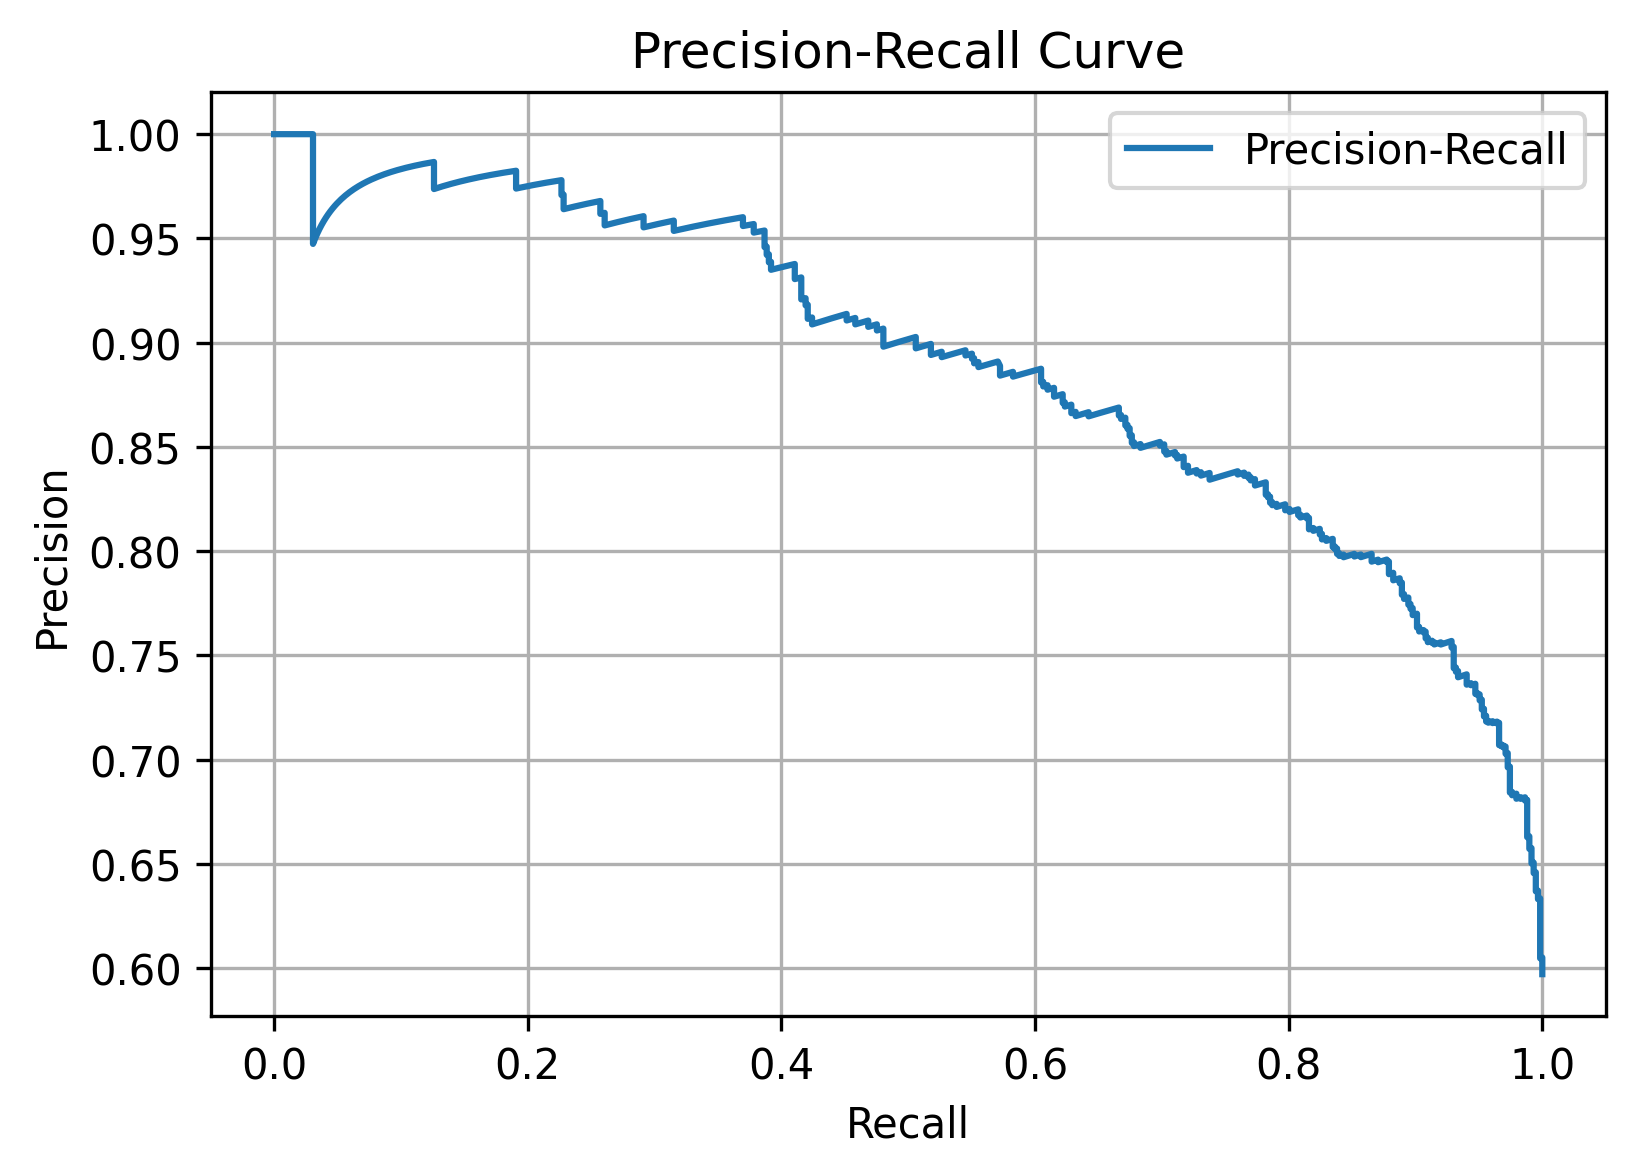
\includegraphics[width=0.5\textwidth]{graph_precision_recall.png}
\caption{Precision-Recall Curve for the Home-Win Class.}
\label{fig:precision_recall}
\end{figure}

\noindent
\textbf{Precision-Recall Analysis.}
Precision is defined as \(\text{TP} / (\text{TP} + \text{FP})\), and recall is \(\text{TP} / (\text{TP} + \text{FN})\). This plot is especially relevant when the cost of false positives vs.\ false negatives differs. We see that precision remains relatively high for a wide range of recall levels, which is beneficial if the application requires capturing most home-team wins (high recall) without incurring too many false positives. As recall approaches 1.0, precision naturally declines, illustrating the trade-off between these two metrics.

\subsection{Prediction vs.\ Actual Point Differential}

\begin{figure}[H]
\centering
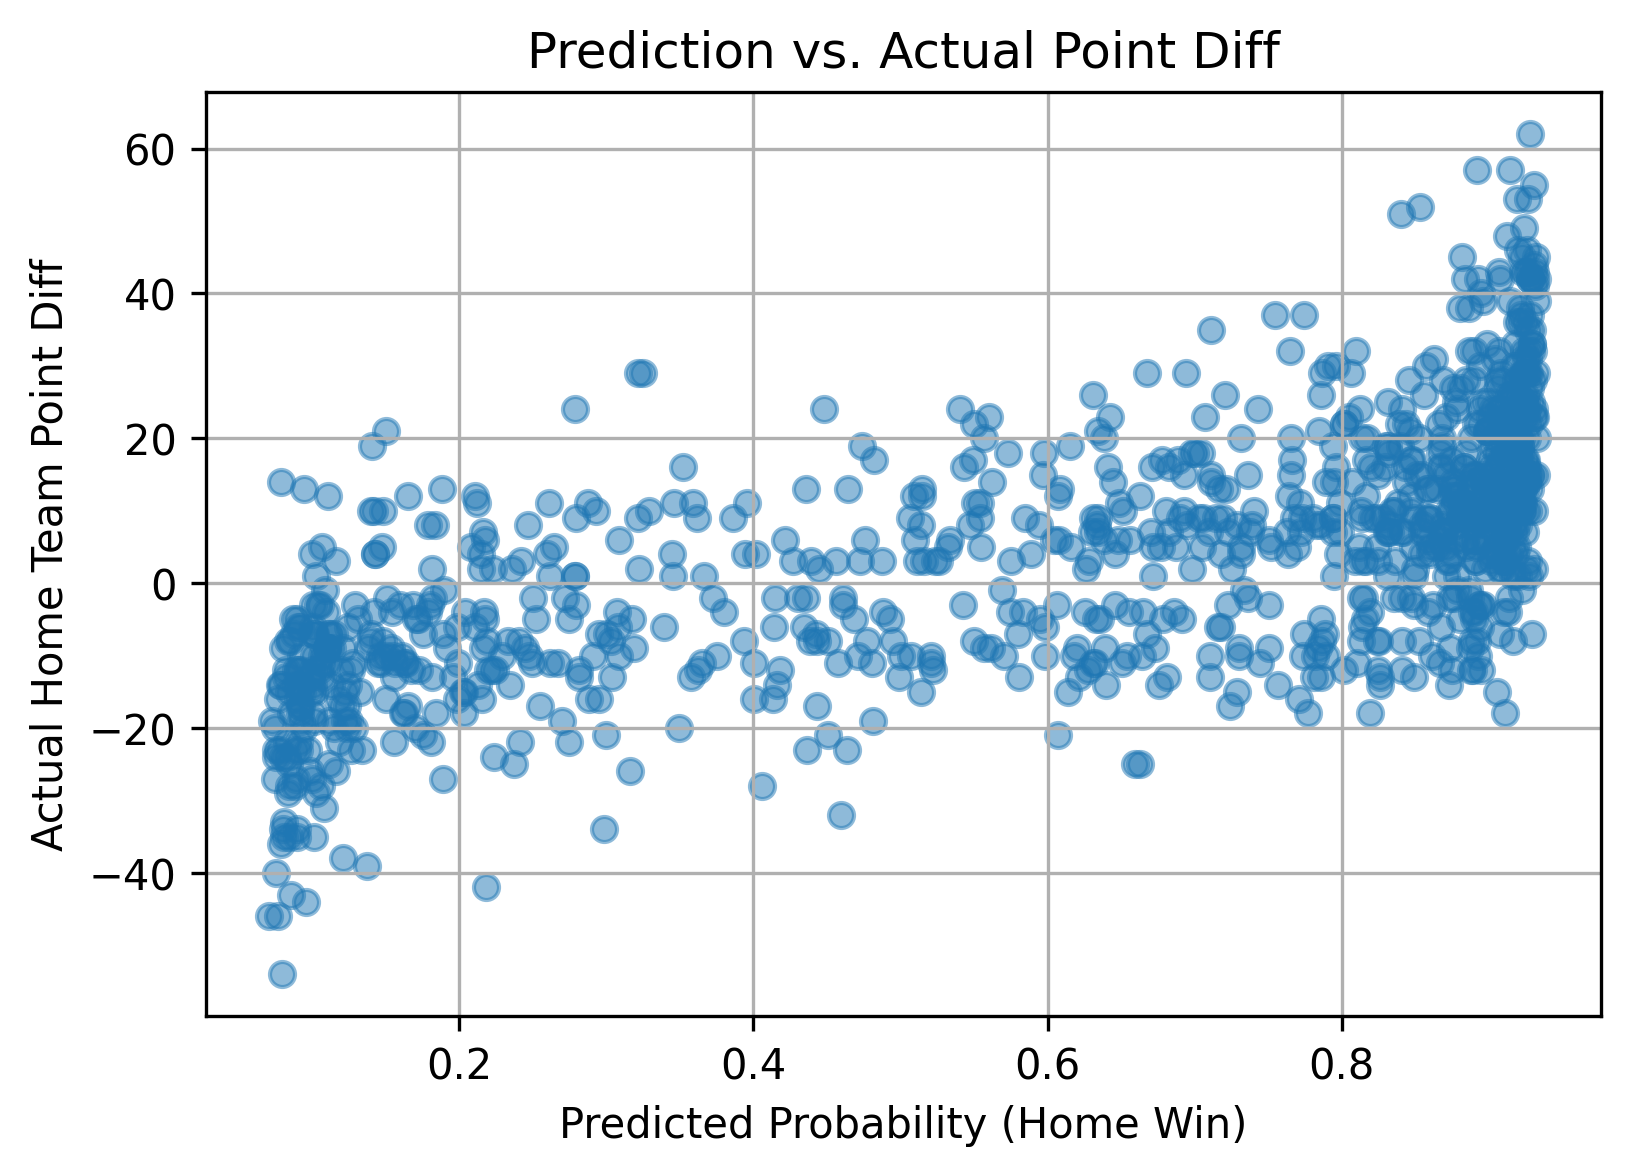
\includegraphics[width=0.5\textwidth]{graph_prediction_vs_actual.png}
\caption{Prediction vs.\ Actual Point Differential (home minus away).}
\label{fig:prediction_vs_actual}
\end{figure}

\noindent
\textbf{Precision-Recall and Point Differential Analysis.}
The scatter plot indicates a strong correlation between the model’s predicted probability of a home-team win (x-axis) and the actual margin of victory or loss (y-axis). As predicted probabilities approach 1.0, the actual home-team point differential is often significantly positive (large margin of victory). Conversely, when predicted probabilities fall below 0.5, we observe many negative point differentials, indicating away-team success. This correlation shows that the model captures not just the binary outcome but also the \emph{degree} of dominance in many cases.

\subsection{Summary of Model Performance}

\paragraph{Overall Metrics.}
Beyond accuracy (\(\approx 79\%\)) and ROC AUC (0.855), the model’s calibration is quantified by a low Brier Score (0.1523) and a well-aligned calibration curve. Together, these metrics suggest that:
\begin{itemize}
    \item The model is \emph{discriminative}, effectively separating home and away wins (high AUC).
    \item The model is \emph{well-calibrated}, meaning its predicted probabilities match actual outcome frequencies.
\end{itemize}

\paragraph{Conclusion.}
By leveraging a stacking ensemble of XGBoost and Random Forest with a Logistic Regression meta-learner, alongside carefully engineered features (including difference/ratio stats, strength-of-schedule, rest days), we achieve a model that excels in both \emph{accuracy} and \emph{calibration}.
\end{document}
